% Тут используется класс, установленный на сервере Papeeria. На случай, если
% текст понадобится редактировать где-то в другом месте, рядом лежит файл matmex-diploma-custom.cls
% который в момент своего создания был идентичен классу, установленному на сервере.
% Для того, чтобы им воспользоваться, замените matmex-diploma на matmex-diploma-custom
% Если вы работаете исключительно в Papeeria то мы настоятельно рекомендуем пользоваться
% классом matmex-diploma, поскольку он будет автоматически обновляться по мере внесения корректив
%

% По умолчанию используется шрифт 14 размера. Если нужен 12-й шрифт, уберите опцию [14pt]
%\documentclass[14pt]{matmex-diploma}
\documentclass[14pt]{matmex-diploma-custom}

\usepackage{tocvsec2}
\usepackage{amssymb}
\usepackage{listings}

\usepackage{xcolor}
\usepackage[font=small,labelsep=period]{caption}

% Calligraphy letters
% use: \mathcal
\usepackage[mathscr]{eucal}
% Algorithms
% use: \begin{algorithm}
\usepackage{algorithm}
% use: \begin{algorithmic}
\usepackage[noend]{algpseudocode}
% Maths
% use: for correct control sequence
\usepackage{amsmath}
% Centreing
% use: \centering
\usepackage{varwidth}
% First indent
% use: automatically
\usepackage{indentfirst}

\definecolor{bluekeywords}{rgb}{0,0,1}
\definecolor{greencomments}{rgb}{0,0.5,0}
\definecolor{redstrings}{rgb}{0.64,0.08,0.08}
\definecolor{xmlcomments}{rgb}{0.5,0.5,0.5}
\definecolor{types}{rgb}{0.17,0.57,0.68}

\lstset{
    inputencoding=utf8x, 
    extendedchars=false, 
    keepspaces = true,
    language=[Sharp]C,
    captionpos=b,
    frame=lines, % Oberhalb und unterhalb des Listings ist eine Linie
    showspaces=false,
    showtabs=false,
    breaklines=true,
    showstringspaces=false,
    breakatwhitespace=true,
    escapeinside={(*@}{@*)},
    commentstyle=\color{greencomments},
    morekeywords={partial, var, value, get, set},
    keywordstyle=\color{bluekeywords},
    stringstyle=\color{redstrings},
    basicstyle=\footnotesize\ttfamily,
}


\renewcommand{\lstlistingname}{Листинг}

\newtheorem{Th}{Теорема}[section]
\newtheorem{Def}{Определение}[section]
\newtheorem{Lem}{Утверждение}[subsection]

\newcommand{\underdot}[1]{\mathop{#1}\limits_{\cdot}}

\newenvironment{Proof} % имя окружения
{\par\noindent{\bf Доказательство.}} % команды для \begin
{\hfill$\scriptstyle\blacksquare$} % команды для \end

\newcommand\abs[1]{\left|#1\right|}
\newcommand\absBigg[1]{\Biggl|#1\Biggr|}

\newcommand{\Pc}{\mathbf{P}_\mathrm{c}}
\newcommand{\In}{\mathbf{I}_n}
\newcommand{\PcHat}{\mathbf{\widehat{P}}_\mathrm{c}}
\newcommand{\PcEv}{\mathbf{P}_\mathrm{c}^{\mathrm{ev}}}

\newcommand{\evidence}{\langle c_{i}, c_{j} \rangle}
\newcommand{\evidenceNumbersGind[1]}{\langle \mathrm{GInd}(#1,m),\mathrm{GInd}(\powTwo-#1,m)\rangle}
\newcommand{\evidenceNumbers}{\langle i, j \rangle}

\newcommand{\redistributor}{\mathbf{r}^{\evidenceNumbers}}
\newcommand{\redistributorGInd[1]}{\mathbf{r}^{\evidenceNumbersGind[#1]}}

\newcommand{\deltaP}{d\left(p,\widehat{p}\right)}

\newcommand{\powTwo}{2^{n^{'}}-1}

\newcommand\p{p}
\newcommand\pHat{\widehat{p}}

\newcommand\probability[1]{p\left(#1\right)}
\newcommand\probabilityHat[1]{p\left(#1\right)}


\newcommand{\PVector}[1]{\mathbf{P}_\mathrm{#1}}

\newcommand{\IFirst}{\mathbf{I}_1}

\newcommand{\Jn}{\mathbf{J}_n}
\newcommand{\JFirst}{\mathbf{J}_1}

\newcommand{\Ln}{\mathbf{L}_n}
\newcommand{\Kn}{\mathbf{K}_n}
\newcommand{\HMatrix}{\mathbf{H}}
\newcommand{\Hij}{\HMatrix^{\evidenceNumbers}}

\newcommand{\Pq}{\PVector{q}}
\newcommand{\Pd}{\PVector{d}}
\newcommand{\PdApost}{\PVector{d}^{'}}
\newcommand{\PdijApost}{\PVector{d}^{', \evidenceNumbers}}

\newcommand{\Pcicj}{p\evidence}

\newcommand{\Tij}{\mathbf{T}^{\evidenceNumbers}}
\newcommand{\TijTilda}{\widetilde{\mathbf{T}}^{\evidenceNumbers}}

\newcommand{\squareMatrix}[2]{\begin{pmatrix} #1 \\ #2 \end{pmatrix}}

\newcommand{\TPlusMatrix}{\squareMatrix{0 & 1}{0 & 1}}
\newcommand{\TMinusMatrix}{\squareMatrix{1 & -1}{0 & 0}}
\newcommand{\TZeroMatrix}{\squareMatrix{1 & 0}{0 & 1}}


\newcommand{\HPlusMatrix}{\squareMatrix{0 & 0}{0 & 1}}
\newcommand{\HMinusMatrix}{\squareMatrix{1 & 0}{0 & 0}}
\newcommand{\HZeroMatrix}{\squareMatrix{1 & 0}{0 & 1}}

\newcommand{\Mij}{\mathbf{M}^{\evidenceNumbers}}
\newcommand{\MijTilda}{\widetilde{\mathbf{M}}^{\evidenceNumbers}}

\newcommand{\MPlusMatrix}{\squareMatrix{1 & -1}{0 & 0}}
\newcommand{\MMinusMatrix}{\squareMatrix{0 & 1}{0 & 1}}
\newcommand{\MZeroMatrix}{\squareMatrix{1 & 0}{0 & 1} }

\newcommand{\Pij}{\mathbf{P}^{\evidenceNumbers}}
\newcommand{\Pijc}{\PVector{c}^{\evidenceNumbers}}
\newcommand{\Pijq}{\PVector{q}^{\evidenceNumbers}}

\newcommand{\dij}{\mathbf{d}^{\evidenceNumbers}}
\newcommand{\dijTilda}{\widetilde{\mathbf{d}}^{\evidenceNumbers}}

\newcommand{\dPlusMatrix}{\squareMatrix{1}{-1}}
\newcommand{\dMinusMatrix}{\squareMatrix{0}{1}}
\newcommand{\dZeroMatrix}{\squareMatrix{1} {0}}

\newcommand{\rij}{\mathbf{r}^{\evidenceNumbers}}
\newcommand{\rijTilda}{\widetilde{\mathbf{r}}^{\evidenceNumbers}}

\newcommand{\rPlusMatrix}{\squareMatrix{0} {1}}
\newcommand{\rMinusMatrix}{\squareMatrix{1}{-1}}
\newcommand{\rZeroMatrix}{\squareMatrix{1}{0}}

\newcommand{\sij}{\mathbf{s}^{\evidenceNumbers}}
\newcommand{\sijTilda}{\widetilde{\mathbf{s}}^{\evidenceNumbers}}

\newcommand{\sPlusMatrix}{\squareMatrix{0}{1}}
\newcommand{\sMinusMatrix}{\squareMatrix{1}{0}}
\newcommand{\sZeroMatrix}{\squareMatrix{1}{1}}

\graphicspath{{Graphs/}}
 
\begin{document}
% Год, город, название университета и факультета предопределены,
% но можно и поменять.
% Если англоязычная титульная страница не нужна, то ее можно просто удалить.
\filltitle{ru}{
    chair              = {Направление <<Математическое обеспечение и администрирование информационных систем>> \\ Профиль <<?>>},
    title              = {Алгебраические байесовские сети: синтез глобальных структур и алгоритмы логико-вероятностного вывода \\(проектная работа)},
    %   master - Диплом магистра
    %   bachelor - Диплом бакалавра
    type               = {master},
    position           = {студента},
    group              = 646,
    author             = {Екатерина Андреевна Мальчевская},
    supervisorPosition = { проф.\,каф.\,инф.,\,д.\,ф.-м.\,н.,\,доц.},
    supervisor         = {Тулупьев А.\,Л.},
    reviewerPosition   = {?},
    reviewer           = {? },
    chairHeadPosition  = {д.\,ф.-м.\,н., профессор},
    chairHead          = {? К.\,Х.},
%   university         = {Санкт-Петербургский Государственный Университет},
%   faculty            = {Математико-механический факультет},
%   city               = {Санкт-Петербург},
%   year               = {2013}
}
\filltitle{en}{
    chair              = {Mathematical Software and Information Systems Administration \\ ??},
    title              = {Empty subset as closed set},
    author             = {Ekaterina Malchevskaia},
    supervisorPosition = {Professor,\,PhD,\,Associate Professor},
    supervisor         = {Tulupyev A. L.},
    reviewerPosition   = {?},
    reviewer           = {?},
    chairHeadPosition  = {professor},
    chairHead          = {Christobal Junta},
}
\maketitle
\tableofcontents
% У введения нет номера главы
 
    % Introduction
    %%%%%%%%%%%%%%%%%%%%%%%%%%%%%%%%%%%%%%%
    \section*{Введение}

\underline{Актуальность темы.} Алгебраические байесовские сети~(АБС), являющиеся одним из классов вероятностных графических моделей, позволяют обрабатывать данные с неопределенностью, которая может порождаться, как необходимостью трансформации высказываний с естественного языка на математический (например высказывания ``скорее всего'', ``наверное'', ``возможно'' удобнее представлять интервальной оценкой вероятности чем скалярной), так и возникновением пробелов в собранных и анализируемых данных. Возможность работать с неопределенностью различного рода в данных является одним из преимуществ алгебраических байесовских сетей в сравнении с другими родственными им вероятностными графическими моделями, в частности с байесовскими сетями доверия, которые не позволяют обрабатывать интервальные оценки вероятности истинности.
   
   Понятие алгебраических байесовских сетей было введено В.И.~Городецким в 1993 году. С того момента теория существенно развивалась, были написаны работы по различным ветвлениям теории: структурному представлению алгебраических байесовских сетей, глобальному и локальному логико-вероятностному выводу.
   %уточняющие и дополняющие срез теории АБС, связанный со структурными представлениями, например первичными и вторичными структурами~\cite{struct1,struct2}. Также были написаны работы, рассматривающие и развивающие подходы к логико-вероятностному выводу в АБС~(поддержание непротиворечивости, априорный вывод, апостериорный вывод)~\cite{consist1,aprior1,apost1,apost2,matr}.
   
   %
   %Расширить
   Упомянутый раньше логико-вероятностный вывод~(ЛВВ) является основным математическим аппаратом, с помощью которого осуществляется обработка существующих данных и получение новых в теории АБС. Эта машина вывода подразделяется на проверку и поддержание непротиворечивости, решение задач априорного и апостериорного вывода. Машина может воздействовать на разных уровнях сети: на локальном и глобальном. `Глобальный'' говорит нам о том, что в область нашего рассмотрения попадает вся сеть и входящие в нее ФЗ, а ``локальный'' о том, что область рассмотрения сужается до одного фрагмента знаний.
        
     Ранее в рамках обширного проекта по работе с АБС AlgBN Web App на языке программирования C\# была спроектирован и реализован комплекс программ, математическая библиотека AlgBN Math Library, позволяющая создавать локальные структуры АБС и выполнять над ними локальный ЛВВ. В дальнейшем планируется использование библиотеки в еще одной составной части проекта -- комплексе программ по работе с различными глобальными структурами АБС (первичной, вторичной, третичной...). Для этого необходимо было спроектировать и реализовать контракт для внешнего доступа и удобного использования функциональности библиотеки.  
     
     Как один из способов анализа алгоритмов локального логико-вероятностного вывода, требовалось посчитать оценку чувствительности при некоторых начальных условиях и выбранной вариации одной величины. Было решено рассмотреть анализ чувствительности первой задачи локального апостериорного вывода с детерминированным свидетельством для фрагмента знаний со скалярными оценками и вариацией оценок вероятности исходного вектора. 
  % Магистерская диссертация базируется на бакалаврской !!!!!
        
        \underline{Объектом исследования} являются алгебраические байесовские сети, а \underline{предметом исследования} -- локальный логико-вероятностный вывод в АБС с использованием матрично-векторных алгоритмов.
        
        \underline{Целью данной магистерской диссертации} является реинжениринг библиотеки для осуществления локального логико-вероятностного вывода над фрагментами знаний AlgBN Math Library. Для достижения поставленной цели были сформированы \underline{задачи}:
            \begin{enumerate}
                \item[1)] разработать систему Unit-тестов для библиотеки AlgBN Math Library;
                \item[2)] спроектировать и реализовать настройку в AlgBN Math Library для осуществления локального ЛВВ в применении в глобальных структурах;
                \item[3)] внедрить парсер в машину для априорного вывода в AlgBN Math Library;
                \item[4)] реализовать систему методов для проведения вычислительных экспериментов по вычислению оценки чувствительности первой задачи для детерминированного свидетельства и ФЗ со скалярными оценками в AlgBN Math Library.
            \end{enumerate}
        
        \underline{Апробация результатов исследования.} Результаты исследования были представлены на восьми научных конференциях.
        
        \underline{Публикации.} По теме магистерской диссертации было опубликовано 15 научных трудов.
        
       \bigskip
         {\small Эта работа является частью более широких инициативных проектов, выполняющихся в лаборатории теоретических и междисциплинарных основ информатики СПИИРАН под руководством А.Л.~Тулупьева; кроме того, разработки были частично поддержаны грантами РФФИ 15-01-09001-a~--- <<Комбинированный логико-вероятностный графический подход к представлению и обработке систем знаний с неопределенностью: алгебраические байесовские сети и родственные модели>>, 18-01-00626~--- <<Методы представления, синтеза оценок истинности и машинного обучения в алгебраических байесовских сетях и родственных моделях знаний с неопределенностью: логико-вероятностный подход и системы графов>>..}
   
    % Chapter 1
    %%%%%%%%%%%%%%%%%%%%%%%%%%%%%%%%%%%%%%%
    \section{Релевантные работы}
\subsection{Введение}
%Базы знаний, декомпозиция, ЛВВ, рисунки, графики неточные вероятности, БСД.


\subsection{Обзор темы исследования}
 Теория вероятностных графических моделей~(ВГМ) являются одной из областей искусственного интеллекта, дающей возможность связать понятия данных, вероятностной логики и теории графов. Соединяя эти понятия исследователь получает возможность анализировать данные, принимая во внимание их связанность между собой (например последовательность состояний или причинно-следственные связи). К ВГМ относятся такие модели как марковские цепи и байесовские сети доверия, которые являются родственными алгебраическим байесовским сетям, являющимися объектом исследования данной работы. Вероятностные графические модели имеют широкое применение в ряде областей и давно подтвердили свою состоятельность, однако АБС выделяются среди прочих ВГМ за счет нескольких факторов. Одним из таких факторов  является структура АБС, предполагающая декомпозицию базы знаний на небольшие объемы тесно связанных между собой данных, что позволяет ускорить алгоритмы обработки за счет возможности работы с ограниченным набором элементов. 
 

 
Алгебраические байесовские сети представляются ненаправленными графами с идеалами конъюнктов в узлах. Конъюнктам приписывается либо скалярная~(точечная), либо интервальная оценка вероятности истинности. Назовем идеал конъюнктов с приписанными его элементам оценками вероятности истинности фрагментом знаний~(ФЗ). Фрагмент знаний строится над некоторым множеством атомов. Например для алфавита $A = \{x_1,x_2,x_3\}$  фрагмент знаний будет выглядеть, как на рисунке \ref{KP_3}. 

\begin{figure}[h!]
  \begin{center}
    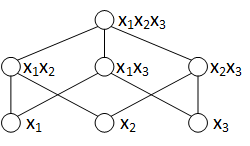
\includegraphics[width=.5\linewidth]{Conj_3_KP.png}
    \caption{Фрагмент знаний, построенный над тремя атомами.}
    \label{KP_3}
  \end{center}
\end{figure}


%Переделать АБС на с большим количеством ФЗ
На рисунке \ref{ABN} изображена алгебраическая байесовская сеть, состоящая из двух фрагментов знаний.

\begin{figure}[h!]
  \begin{center}
    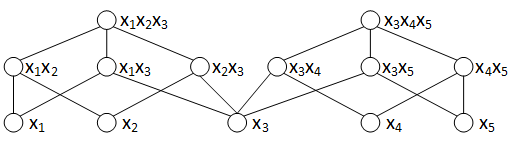
\includegraphics[width=.9\linewidth]{ABN_2.png}
    \caption{АБС, состоящая из двух фрагментов знаний.}
    \label{ABN}
  \end{center}
\end{figure}
    
Основным аппаратом для обработки существующих и получения новых знаний является логико-вероятностный вывод~(ЛВВ)~\cite{nsmv}. По уровню действия на сеть логико-вероятностный вывод делится на глобальный и локальный. ``Глобальный'' говорит нам о том, что в область нашего рассмотрения попадает вся сеть и входящие в нее ФЗ, а ``локальный'' о том, что область рассмотрения сужается до одного фрагмента знаний. Задачи, рассматриваемые в ЛВВ, включают в себя проверку непротиворечивости, поддержание непротиворечивости (для случая интервальных оценок), задачу априорного вывода и две задачи апостериорного вывода. 
    
В глобальном случае при проверке и поддержке непротиворечивости в сети, оценки вероятности истинности элементов сети проверяются на согласованность и, при возможности, уточняются. В локальном случае мы рассматриваем и работаем только с одним зафиксированным ФЗ из сети и проверяем на согласованность и пытаемся уточнить оценки только в нем, не затрагивая при этом остальные ФЗ сети. 
    
Априорный вывод~\cite{tul} заключается в том, что мы оцениваем вероятность истинности пропозициональной формулы, построенной над каким-то фиксированным алфавитом. В локальном виде вывода формула строится над тем же алфавитом, что и рассматриваемый ФЗ.
    
Задачи апостериорного вывода возникают тогда, когда в нашу сеть поступает новая обуславливающая информация, которую мы будем называть свидетельством. В глобальном случае свидетельство поступает во всю сеть и строится над алфавитом сети, а в локальном -- в выбранный ФЗ и строится над его алфавитом. Первая задача апостериорного вывода сводится к вычислению вероятности свидетельства на основе оценок вероятности истинности, заданных во фрагменте знаний. Вторая задача состоит в вычислении условных оценок вероятности истинности во фрагменте знаний с учетом поступившего свидетельства. В рамках теории алгебраических байесовских сетей разделяют три вида свидетельств: детерминированное, стохастическое и неточное. Детерминированное свидетельство является базовым и наиболее простым и операции с более сложными видами свидетельств так или иначе сводятся к детерминированному случаю. В глобальных операциях над сетью используются локальные операции, то есть обработка конкретных фиксированных ФЗ. Поэтому так важно изучение и развитие именно локального вывода и, в частности, апостериорного вывода с использованием детерминированного свидетельства, который будет рассмотрен в данной работе. 
    
Анализ чувствительности является одним из критериев оценки математической модели~\cite{WOS5_sensitivity,WOS2_sensitivity,WOS6_sensitivity}. Характеризуя степень колебания результата в зависимости от изменения входных данных, чувствительность имеет практическое предназначение и позволяют определить степень претенциозности к точности входных данных, что сказывается на количестве входных данных необходимых на вход соответствующему алгоритму для получения результата заданной точности.    

%ссылки из СЕЙМ и ИИТИ17

\subsection{Выводы по главе}




    % Chapter 2
    %%%%%%%%%%%%%%%%%%%%%%%%%%%%%%%%%%%%%%%
    \section{Основные термины, объекты и результаты в теории логико-вероятностного вывода в теории алгебраических байесовских сетей}
\subsection{Введение}

\subsection{Модель ФЗ}
	\subsubsection{ФЗ, построенные над идеалом конъюнктов}
	Алгебраическая байесовская сеть является одной из моделей, которые представляют данные с неопределенностью, а также вероятностной графической моделью. Неопределенность возникает вследствие того, что конъюнктам в узлах фрагментов знаний, из которых состоит АБС, приписывается некоторая вероятность, степень неточности. 
          
           \begin{Def}
            ~\cite{AVS_2011}
                Алфавит А $= \{ x_{i}\}^{n - 1}_{i = 0}$ -- конечное множество атомарных пропозициональных формул (атомов). Введем нумерацию атомов с нуля.
            \end{Def}


           Над атомами из указанного алфавита определим  наборы пропозициональных формул.
            
            \begin{Def}
            ~\cite{AVS_2011}
                Конъюнкт (цепочка конъюнкций) -- это конъюнкция некоторого числа атомарных переменных вида:
                \begin{eqnarray*}
                    x_{i_{1}} \wedge x_{i_{2}} \wedge \cdots \wedge x_{i_{k}}.
                \end{eqnarray*}
            \end{Def}
            
 
            Теперь введем некоторые определения, связанные с видами фрагментов знаний.
        
            \begin{Def}
                ~\cite{AVS_2011}
                Фрагмент знаний (ФЗ) со скалярными оценками -- это пара вида \begin{math}(C,p)\end{math}, где \begin{math}C\end{math} -- идеал конъюнктов, а \begin{math}p\end{math} --  функция из \begin{math}C\end{math} в интервал  
                \begin{math}
                [0;1]
                \end{math}
            \end{Def}
         
            \begin{Def}
            ~\cite{AVS_2011}
                Фрагмент знаний (ФЗ) с интервальными оценками -- это структура вида \begin{math}(C,p)\end{math}, где \begin{math}C\end{math} -- идеал конъюнктов, а \begin{math}p\end{math} --  функция из \begin{math}C\end{math} в множество интервалов вида 
                \begin{eqnarray*}
                    \{[a;b] : a, b \in [0;1], a \leq b\}.
                \end{eqnarray*}
            \end{Def}
           
           Оценки вероятности истинности, приписанные элементам ФЗ, организуются в один или два вектора $\mathbf{P_{c}}$ и $\{\mathbf{P_{c}^{-}}, \mathbf{P_{c}^{+}}\}$ соответственно. Вектор $\mathbf{P_{c}}$ задается при скалярных оценках. Векторы $\{\mathbf{P_{c}^{-}}, \mathbf{P_{c}^{+}}\}$ задаются при интервальных оценках. В последнем случае в один из векторов ($\mathbf{P_{c}^{-}}$) помещаются нижние границы оценок, а в другой ($ \mathbf{P_{c}^{+}}$) -- верхние границы. 
    
    \begin{eqnarray*}
        \mathbf{P_{c}} = \left( \begin{array}{c}
            1 \\
            p(c_{1}) \\
            \vdots \\
            p(c_{2^{n-1}})
        \end{array}  \right)
    \end{eqnarray*}
    \begin{eqnarray*}
        \mathbf{P_{c}^{-}} = \left( \begin{array}{c}
            1 \\
            p^{-}(c_{1}) \\
            \vdots \\
            p^{-}(c_{2^{n -1}})
        \end{array}  \right); 
        \mathbf{P_{c}^{+}} = \left( \begin{array}{c}
            1 \\
            p^{+}(c_{1}) \\
            \vdots \\
            p^{+}(c_{2^{n -1}})
        \end{array}  \right).
    \end{eqnarray*}
    
            Введем определения непротиворечивости и согласуемости ФЗ~\cite{AVS_2011}.
            
               
            \begin{Def}
            ~\cite{AVS_2011}
                 Пусть задан ФЗ со скалярными оценками вероятности \begin{math}(C,p)\end{math}. Мы говорим, что он непротиворечив(согласован), и обозначаем это как \begin{math}\mathrm{Consistent}[(C,p)]\end{math} тогда и только тогда, когда существует вероятность \begin{math}p_{F}\end{math}, заданная над множеством пропозициональных формул \begin{math}F(A)\end{math}(где \begin{math}A\end{math} -- это алфавит, над которым построен ФЗ), такая что 
                \begin{eqnarray*}
                    \forall c\in C \:  p_{F} = p(c).
                \end{eqnarray*}
            \end{Def}
          
            \begin{Def}
            ~\cite{AVS_2011}
                Пусть задан ФЗ с интервальными оценками вероятности \begin{math}(C,p)\end{math}. Мы говорим, что он \it{непротиворечив}(согласован), и обозначаем это как \begin{math}\mathrm{Consistent}[(C,p)]\end{math} тогда и только тогда, когда для любого конъюнкта \begin{math} c \in C \end{math}  и любого \begin{math} \epsilon \in p(c) \end{math} найдется функция \begin{math} p_{c,\epsilon} : C \to [0,1] \end{math}  такая, что \begin{math} p_{c,\epsilon} = \epsilon \end{math} и \begin{math} (C, p_{c,\epsilon}) \end{math} -- непротиворечивый в смысле предыдущего определения.
            \end{Def}
            
            \begin{Def}
            ~\cite{AVS_2011}
                Пусть задан ФЗ с интервальными оценками вероятностей \begin{math}(C,p)\end{math}. Мы говорим, что он \it{согласуем} тогда и только тогда, когда существует непротиворечивый ФЗ с интервальными оценками \begin{math}(C,p')\end{math} такой, что 
                \begin{eqnarray*}
                    \forall c\in C \:  p'(c) \subseteq p(c).
                \end{eqnarray*}
            \end{Def}
            
            
            Введем основные понятия локального апостериорного логико-ве\-роят\-ност\-но\-го вывода в рамках рассматриваемой модели ФЗ. Для формализации локального логико-вероятностного вывода нам необходимо ввести определение математической модели свидетельства в АБС.

            \begin{Def}
            ~\cite{AVS_2011}
                Задача локального априорного вывода состоит в том, чтобы на основе непротиворечивого фрагмента знаний построить оценки истинности пропозициональной формулы, заданной над тем же алфавитом, что и фрагмент знаний.
            \end{Def}

            % Свидетельство  

            \begin{Def}
            ~\cite{AVS_2011}
                Свидетельство -- новые <<обусловливающие>> данные, которые поступили во ФЗ, и с учетом которых нам требуется пересмотреть все (или только некоторые) оценки. Для обозначения свидетельства будут использоваться угловые скобки -- $\langle \cdots \rangle$.
            \end{Def}
            
            Далее оговорим, что из себя представляют задачи апостериорного логико-вероятностного вывода.
            
            % Задачи апостериорного вывода

            \begin{Def}
            ~\cite{AVS_2011}
                {\it Первая задача апостериорного вывода} состоит в том, чтобы оценить вероятность истинности свидетельства при уже заданных оценках вероятности истинности элементов ФЗ.
            \end{Def}
            
            \begin{Def}
            ~\cite{AVS_2011}
                {\it Вторая задача апостериорного вывода} состоит в том, чтобы оценить условные вероятности истинности элементов ФЗ при предположении, что имеет место быть свидетельство.
            \end{Def}  
  
    
    \subsection{Алгоритмизация логико-вероятностного вывода}
        Прежде чем приступить непосредственно к рассмотрению алгоритмов решения задач локального логико-вероятностного вывода, разберем аппарат, осуществляющий проверку непротиворечивости вероятностных оценок ФЗ и некоторые понятия с ним связанные.
        
       
            
            Матрица $\mathbf{I}_{n}$, упомянутая ранее, имеет чёткую структуру~\cite{AVS_2011}, которую можно описать рекуррентно.
             $$ \mathbf{I}_{1} = \left( \begin{array}{cc}
                 1 & -1 \\
                 0 &  1 \\
                \end{array}  \right) ,\cdots,\; \mathbf{I}_{n} = \mathbf{I}_{1} \otimes \mathbf{I}_{n-1} = \mathbf{I}_{1} \otimes \mathbf{I}_{1}^{[n-1]} = \mathbf{I}_{1}^{[n]}. $$
                
            При этом выполняется соотношение:
            $$ \mathbf{P_{q}} =  \mathbf{I}_{n} \times \mathbf{P_{c}}. $$
            
            Здесь $\otimes$ кронекерово произведение матриц. Также используется обратная матрице $\mathbf{I}_{n}$ матрица $\mathbf{J}_{n}$, которая удовлетворяет условию:
            \begin{eqnarray*}
                \mathbf{P_{c}} =  \mathbf{J}_{n} \times \mathbf{P_{q}}, \\
                \mathbf{J}_{1} = \left( \begin{array}{cc}
                     1 & 1 \\
                     0 & 1 \\
                \end{array}  \right),\; \mathbf{J}_{n} = \mathbf{J}_{1} \otimes \mathbf{J}_{n-1} = \mathbf{J}_{1} \otimes \mathbf{J}_{1}^{[n-1]} = \mathbf{J}_{1}^{[n]}.
            \end{eqnarray*}
            
            Сформулируем определения непротиворечивости фрагментов знаний, описанные ранее на матрично-векторном языке~\cite{AVS_2011}.
            

            \begin{Def}
                Пусть задан ФЗ со скалярными оценками вероятностей $(C, \mathbf{P_{c}})$. мы говорим, что он непротиворечив тогда и только тогда, когда $$ \mathbf{I}_{n} \times \mathbf{P_{c}} \geq \mathbf{0}.$$
            \end{Def}

            \begin{Def}
                Пусть задан ФЗ с интервальными оценками вероятностей $(C, \mathbf{P^{-}_{c}}, \mathbf{P^{+}_{c}})$. Мы говорим, что он непротиворечив тогда и только тогда, когда 
                \begin{eqnarray*}
                    \forall i : 1 \leq i \leq 2^{n} -1 \qquad \forall \epsilon : \mathbf{P^{-}_{c}}[i] \leq \epsilon \leq \mathbf{P^{+}_{c}}[i]  \\ \exists \mathbf{P_{c}} : 
                    (\mathbf{P^{-}_{c}} \leq \mathbf{P_{c}} \leq \mathbf{P^{+}_{c}})\; \&\; (\mathbf{P_{c}}[i] = \epsilon)\; \&\; (\mathbf{I}_{n} \times \mathbf{P_{c}} \geq 0).
                \end{eqnarray*}
            \end{Def}

            \begin{Def}
                Пусть задан ФЗ с интервальными оценками вероятностей $(C, \mathbf{P^{-}_{c}}, \mathbf{P^{+}_{c}})$. Мы говорим, что он согласуем тогда и только тогда, когда  существует непротиворечивый ФЗ с интервальными оценками $(C, \mathbf{P^{-}}, \mathbf{P^{+}})$, такой что $ \mathbf{P^{-}_{c}} \leq \mathbf{P^{-}}$ и $ \mathbf{P^{+}} \leq \mathbf{P^{+}_{c}}$.
            \end{Def}
            
            Обоснование приведенных выше рассуждений, дополнительные факты, утверждения и теоремы и  примеры приведены в~\cite{AVS_2011}.
            
       
        \subsubsection{Априорный вывод}
            
            Рассмотрим локальный априорный вывод над двумя видами ФЗ: скалярным и интервальным.
            
            \paragraph{Априорный вывод над скалярным ФЗ.}
                Опишем решение задачи априорного вывода для случая ФЗ со скалярными оценками вероятности.
                Рассмотрим непротиворечивый ФЗ со скалярными оценками $(C, \mathbf{P_{c}})$. Мы можем выразить вероятность произвольной пропозициональной формулы через вероятности квантов, входящих в её СДНФ.
                
                \begin{Def}
                    Пусть $f$ -- произвольная пропозициональная формула, тогда характеристическим вектором формулы $f$ мы будем называть вектор $\chi_{f}$, состоящий из $2^{n}$ элементов, такой, что
                
                    \begin{eqnarray*}
                        \chi_{f} [i]
                        =
                        \left \{ 
                            \begin{array}{c}
                            0,\; $если$ \; q_{i} \notin S_{f};  \\
                            1,\; $если$\;  q_{i} \in S_{f}
                        \end{array}\
                        \right.
                    \end{eqnarray*}
                    , где $q_{i}$ обозначает $i$-й квант, а  $S_{f}$ -- множество квантов, содержащихся в СДНФ ф-лы $f$.
                \end{Def}
                
                
                Рассмотрим пропозициональную формулу $f$, истинность которой требуется оценить. На основе прежде рассмотренных знаний мы можем сделать вывод, что 
                $$ p(f) = (\chi_{f}, \mathbf{P_{q}}).$$
                
                Используя ранее рассмотренные формулы, мы можем перейти от вектора с вероятностями квантов к вектору с вероятностями конъюнктов и получим
                 \begin{eqnarray*}
                    p(f) = (\chi_{f}, \mathbf{I}_{n} \times \mathbf{P_{c}}) = (\mathbf{I}_{n}^ {\mathbf{T}} \times \chi_{f}, \mathbf{P_{c}}).
                \end{eqnarray*}
                Обозначим $\mathbf{L_{f}} = \mathbf{I}_{n}^{{T}} \times \chi_{f}$, тогда 
                \begin{eqnarray*}
                    p(f) = (\mathbf{L_{f}}, \mathbf{P_{c}}).
                \end{eqnarray*}
 
            
            \paragraph{Априорный вывод над интервальным ФЗ.}
                Перейдем к ФЗ с интервальными оценками вероятности. В данном случае однозначно определить вероятность истинности пропозициональной формулы не удастся, но можно найти максимальную и минимальную оценки:
                 \begin{eqnarray*}
                     p^{-}(f) =
                     \displaystyle \min_{\mathfrak{D}\cup \mathfrak{E}}
                     (\mathbf{L_{f}}, \mathbf{P_{c}}), \qquad
                     p(f)^{+} = 
                     \displaystyle \max _{\mathfrak{D}\cup \mathfrak{E}}
                     (\mathbf{L_{f}}, \mathbf{P_{c}}).
                \end{eqnarray*}
 
        
        \subsubsection{Апостериорный вывод}
            В теории АБС рассматриваются три вида свидетельств: детерминированные, стохастические и неточные.
            
            % Виды свидетельств

            \begin{Def}
                {\it Детерминированное свидетельство} -- некоторое означивание цепочки конъюнкций, рассматриваемое в качестве поступившего свидетельства. Данное свидетельство обозначается \begin{math} \langle c_{i}, c_{j} \rangle \end{math}. Здесь \begin{math}c_{i}, c_{j}\end{math} -- конъюнкты, состоящие из атомов, получивших положительные и отрицательные означивания соответственно.
            \end{Def}             

            \begin{Def}
                {\it Стохастическое свидетельство} -- непротиворечивый ФЗ, заданный над \begin{math} C'\end{math} -- подыдеале \begin{math} C\end{math}, со скалярными оценками, которые определяет вероятности истинности элементов соответствующего подыдеала. Данное свидетельство обозначается \begin{math} \langle ( C', \mathbf{P_{c}}) \rangle \end{math}.
            \end{Def}           

            \begin{Def}
                {\it Неточное свидетельство} -- непротиворечивый ФЗ с \begin{math} C'\end{math} -- подыдеале \begin{math} C\end{math}  интервальными оценками, которые определяет вероятности истинности элементов соответствующего подыдеала. Данное свидетельство обозначается \begin{math} \langle ( C', \mathbf{P_{c}^{-}},  \mathbf{P_{c}^{+}}) \rangle \end{math}.
            \end{Def}
            
            Все рассмотренные выше задачи образуют локальный логико-ве\-роят\-ност\-ный вывод в АБС, который был реализован в программном комплексе. Также большинство задач ЛВВ сводится к решению задач линейного программирования(ЛП), то есть поиску минимума и максимума некоторой целевой функции, при заданных органичениях, что позволяет использовать известные методы решения задач ЛП.
            
\paragraph{Детерминированное свидетельство  и ФЗ со скалярными оценками.}
            
 Таким образом получим решения первой задачи апостериорного вывода для ФЗ над идеалом конъюнктов~\cite{tulupex2015rus}:
\begin{equation*}
    \Pcicj = (\rij, \Pc),
\end{equation*}
причем
\begin{math} \rij = \rijTilda_{n - 1} \otimes \rijTilda_{n - 2} \otimes \cdots \otimes \rijTilda_0 \quad
    \rijTilda_{k} = \begin{cases}
   \mathbf{r}^+ \text{, если $x_k$ входит в $c_i$}\\
   \mathbf{r}^- \text{, если $x_k$ входит в $c_j$}\\
   \mathbf{r}^0 \text{, иначе}
 \end{cases}
\end{math},
\begin{math}
    \mathbf{r}^+ = \rPlusMatrix; \qquad \mathbf{r}^- = \rMinusMatrix; \qquad \mathbf{r}^0 = \rZeroMatrix
\end{math}


 %Слова про то, что рассмотрим только эту формулу. остальные можно найти -- там-то.           
                
                
                
\subsection{Чувствительность первой задачи апостериорного вывода}

 Анализ чувствительности является одним из критериев оценки математической модели \cite{WOS5,WOS2}. Данная оценка характеризует степень изменения результата в зависимости от колебания значений входных данных.
    
    В работе \cite{iiti2017} была сформирована следующая задача линейного программирования~(ЗЛП) для оценки чувствительности первой задачи апостериорного вывода:
            \begin{equation*}
            \varepsilon(\Pc^{\circ}) = \max_{\substack{
            \PcHat\In \geq 0, \Pc^{\circ}\In \geq 0,\\ 
            v(\Pc^{\circ}, \PcHat)\leq\delta,\\ 
            \p\evidence=(\redistributor,\Pc^{\circ}),\\ 
            \pHat\evidence=(\redistributor,\PcHat)}}
            {\{\p-\pHat, \pHat-\p\}}.
            \end{equation*}
            
    С целью исследования поведения оценки чувствительности первой задачи апостериорного вывода для детерминированного свидетельства при колебании входных оценок вероятности истинности элементов исходного ФЗ, были проведены вычислительные эксперименты, описанные далее.
    
\subsection{Выводы по главе}
    
    % Chapter 3
    %%%%%%%%%%%%%%%%%%%%%%%%%%%%%%%%%%%%%%%
    \section{Результаты теоретического представления данных и основные алгоритмы в библиотеке ЛВВ}
\subsection{Введение}



\subsection{Описание библиотеки, все части}



\subsection{Алгоритм для проведения апостериорного вывода для детерминированного свидетельства}
        
        Рассмотрим алгоритм решения первой и второй задачи апостериорного вывода с использованием вектора-редистрибъютера \cite{AAZ_matr_vect} для детерминированного свидетельства $\evidence$, которое также может быть записано таким образом $\evidenceNumbers$, где $i$ – индекс положительной части, а $j$ – индекс отрицательной. Стоит заметить, что для алфавита, над которым строится свидетельство, индекс положительной и отрицательной части является по своей сути маской, которая показывает, какие атому входят в соответствующую часть свидетельства, а какие – нет. В индексе, если атому соответствует 1, то этот атом входит в конъюнкцию атомов определенной части свидетельства, если 0, то нет. 
        
        \begin{lstlisting}[label=list1,caption={Функция GetRedistributerVector},escapeinside={(*}{*)}]
            input:  (*$A = \{x_{n-1} , ... , x_{0}\}, c_i, c_j$*)
            output:  (*$r^{\evidenceNumbers}$*)
            1:   function GenerateRedistributerVector
            2:   	(*$r^{o} = (1,1)$*)
            3:   	(*$r^{+} = (0,1)$*)
            4:   	(*$r^{-} = (1,-1)$*)
            5:	    (*$r^{\evidenceNumbers} = 1$*)
            6:   	foreach (atom in A)
            7:	      	if (atom in (*$c_i$*))
            8:			  (*$r^{\evidenceNumbers}$*)= kroneckerV((*$r^{\evidenceNumbers}$*), (*$r^{+}$*))
            9:	      	else if (atom in (*$c_j$*))
            10:			  (*$r^{\evidenceNumbers}$*)= kroneckerV((*$r^{\evidenceNumbers}$*), (*$r^{-}$*))
            11:	      	else
            12:			  (*$r^{\evidenceNumbers}$*)= kroneckerV((*$r^{\evidenceNumbers}$*), (*$r^{o}$*))
            13:	 return (*$r^{\evidenceNumbers}$*)
        \end{lstlisting}
        
        На листинге \ref{list1} представлена вспомогательная функция GetRedistributer\-Vector для вычисления вектора-редистрибъютера для рассматриваемого свидетельства, на вход которой подается алфавит, над которым задан исходный ФЗ, положительно означенная и отрицательно означенная части свидетельства соответственно. Функция возвращает вычисленный вектор. Здесь и далее запись «atom in A» означает, что atom входит в алфавит A, а запись «atom in » -- atom входит в соответствующую конъюнкцию. Функция kronekerV(t,r) вычисляет кронекерово произведение векторов t и r.
        
        \begin{lstlisting}[label=list2,caption={Функция FirstPosteriorTaskSolution},escapeinside={(*}{*)}]
            input:  (*$A = \{x_{n-1} , ... , x_{0}\}, c_i, c_j, \Pc $*)	
            output:  (*$p(\evidence)$*) 
            1:   function FirstPosteriorTaskSolution
            2:   	  (*$r^{\evidenceNumbers}$*)= GenerateRedistributerVector(A, (*$c_i $*) , (*$c_j $*) )
            3:	    res = 0
            4:   	foreach ( (*$p_i $*) in (*$\Pc $*))
            5:	      foreach ( (*$r_i $*) in (*$r^{\evidenceNumbers}$*) )
            6:		res =  (*$p_i $*) *  (*$r_i $*) 
            7:	 return res
        \end{lstlisting}
        
        На листинге \ref{list2} представлена функция FirstPosteriorTaskSolution для решения первой задачи апостериорного вывода для рассматриваемого свидетельства и исходного ФЗ. На вход поступает алфавит, над которым задан исходный ФЗ, положительно означенная и отрицатель-но означенная части свидетельства и вектор вероятностей истинности элементов ФЗ. Функция возвращает вычисленное значение вероятно-сти.
        
        \begin{lstlisting}[label=list3,caption={Функция GetMatrixT},escapeinside={(*}{*)}]
            input:  (*$A = \{x_{n-1} , ... , x_{0}\}, c_i, c_j$*)	
            output: (*$T^{\evidenceNumbers}$*) 
            1:   function GetMatrixT
            2:   	(*$T^{o} = \left( \begin{array}{cc}
                                1& 0\\  0&1\\  \end{array}  \right)$*)
            3:   	(*$T^{+} = \left( \begin{array}{cc}
                                0& 1\\  0&1\\  \end{array}   \right)$*)
            4:   	(*$T^{-} = \left( \begin{array}{cc}
                                1& -1\\  0&0\\  \end{array}   \right)$*)
            5:	    (*$T^{\evidenceNumbers} = 1$*) 
            6:   	foreach (atom in A)
            7:	      	if (atom in (*$c_i$*))
            8:			 (*$T^{\evidenceNumbers}$*) = kroneckerM((*$T^{\evidenceNumbers}$*), (*$T^{+}$*))
            9:	      	else if (atom in (*$c_j$*))
            10:			 (*$T^{\evidenceNumbers}$*) = kroneckerM((*$T^{\evidenceNumbers}$*), (*$T^{-}$*))
            11:	      	else 
            12:			 (*$T^{\evidenceNumbers}$*) = kroneckerM((*$T^{\evidenceNumbers}$*), (*$T^{o}$*))
            13:	 return (*$T^{\evidenceNumbers}$*)
        \end{lstlisting}
        
        В листинге \ref{list3} приведен псевдокод вспомогательной функции Get\-MatrixT для вычисления матрицы T для рассматриваемого сви\-де\-тель\-ства, на вход которой подается алфавит, над которым задан исходный ФЗ, положительно означенная и отрицательно означенная части свидетельства соответственно. Функция возвращает вычисленную матрицу. Функция kronekerM(T, R) вычисляет кронекерово произведение матриц T и R.
        
        \begin{lstlisting}[label=list4,caption={Функция SecondPosteriorTaskSolution},escapeinside={(*}{*)}]
            input:  (*$A = \{x_{n-1} , ... , x_{0}\}, c_i, c_j, \Pc $*)		
            output:  (*$P_{c}^{\evidenceNumbers}$*)
            1:   function SecondPosteriorTaskSolution
            2:   	 (*$r^{\evidenceNumbers}$*)= GenerateRedistributerVector(A, (*$c_i $*) , (*$c_j $*) )
            3:		 (*$p(\evidence)$*) = FirstPosteriorTaskSolution(A, (*$c_i, c_j, \Pc$*) )
            4:		n = length((*$P_{c}$*))
            5:   	foreach (k in 0:(n-1))
            6:	      	 (*$P_{c}^{\evidenceNumbers}[k] = (r^{\evidenceNumbers}[k] * \Pc [k]) / p(\evidence)$*)
            7:	 return  (*$P_{c}^{\evidenceNumbers}$*)
        \end{lstlisting}
        
        На листинге \ref{list4} представлена функция SecondPosteriorTaskSolution для решения второй задачи апостериорного вывода для рассматриваемого свидетельства и исходного ФЗ. На вход поступает алфавит, над которым задан исходный ФЗ, положительно означенная и отрицательно означенная части свидетельства и вектор вероятностей истинности элементов ФЗ. Функция возвращает вычисленный вектор условных вероятностей истинности конъюнктов ФЗ.



\subsection{ЧТО-ТО}
\subsection{Выводы по главе}

    % Chapter 4
    %%%%%%%%%%%%%%%%%%%%%%%%%%%%%%%%%%%%%%%
    \section{Руководство пользователя и примеры использования}
\subsection{Введение}


\subsection{Общая диаграмма комплекса}
% 	Math net  статья
    
    
\subsection{Надстройка}
%ПЕРЕХОД
Архитектура разработанной надстройки над существующей библиотекой локального логико-вероятностного вывода представлена на диаграмме классов Рис. \ref{Structure}.

\begin{figure}[h!]
\begin{center}
\includegraphics[width=\linewidth]{Structure.png}
\caption{Диаграмма классов расширения библиотеки локального вывода.}
\label{Structure}
\end{center}
\end{figure}

Абстрактный класс BaseKnowledgePattern определяет ту функциональность, которую должны иметь наследующие от него классы: Scalar\-KnowledgePattern и IntervalKnowledgePattern.

Класс ScalarKnowledgePattern реализует расширение фрагмента знаний со скалярными (точечными) оценками вероятности истинности элементов. Он содержит два вида конструктора: одному на вход передается глобальный индекс, другому -- глобальный индекс и массив с оценками вероятности истинности. Имеется отдельный метод для задания оценок элементов ФЗ. Помимо этого, реализованы методы, которые осуществляют поддержание локальной непротиворечивости, решают задачи априорного и апостериорного локального логико-вероятностного вывода. Реализованные методы полностью покрывают требуемую функциональность.

Класс IntervalKnowledgePattern реализует расширение фрагмента знаний с интервальными оценками вероятности истинности элементов. Его методы имеют аналогичную, ранее рассмотренному классу Scalar\-KnowledgePattern, функциональность.


\subsection{Внедрение парсера}

Объемлющий проект AlgBN Web App~\ref{App} по работе с алгебраическими байесовскими сетями включает в себя математическую библиотеку AlgBN Math Library по работе с локальными структурами АБС и осуществлению локального логико-вероятностного вывода над ними.  

\begin{figure}[h!]
\begin{center}
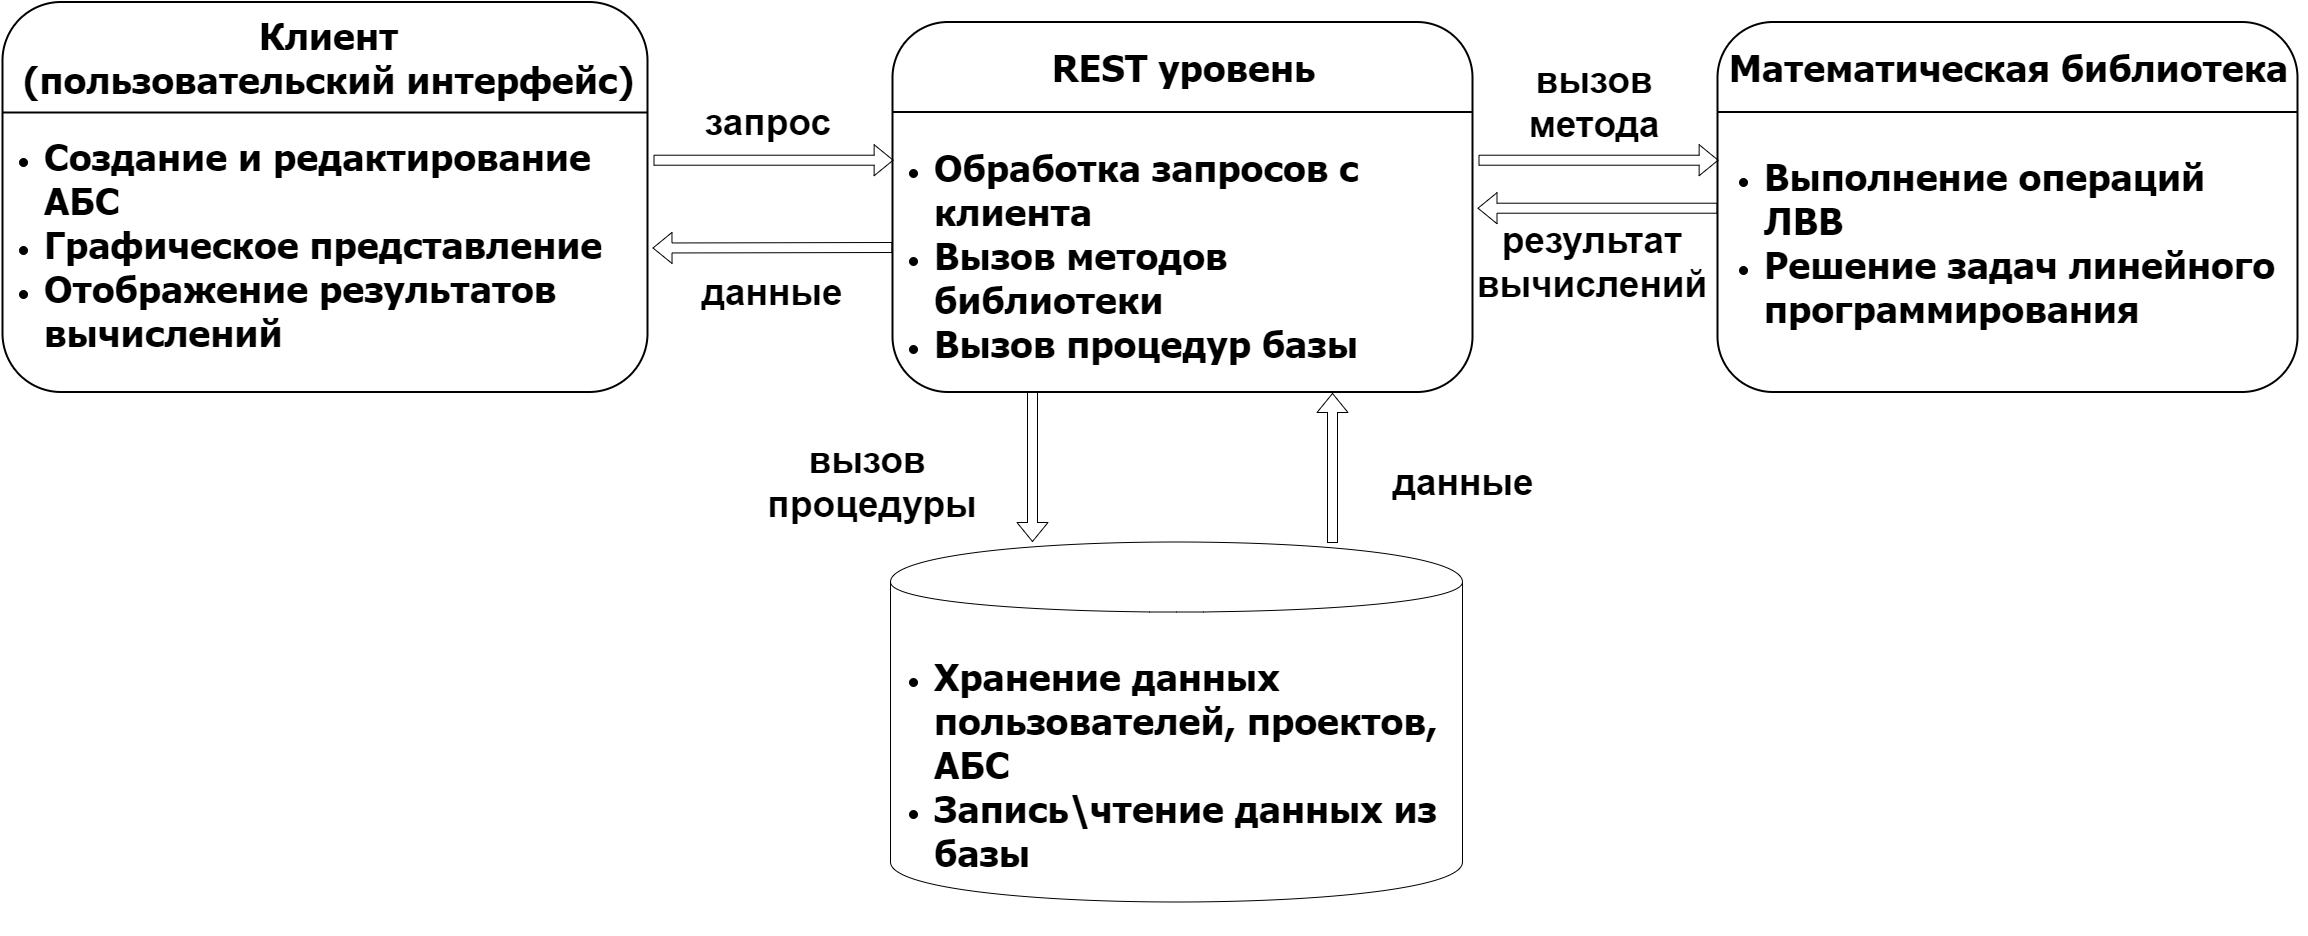
\includegraphics[width=.9\textwidth]{App}
\caption{Диаграмма проекта AlgBN Web App}
\label{App}
\end{center}
\end{figure}

Структура Inferer~\ref{Inf} в библиотеке осуществляет не только проверку и поддержание непротиворечивости во фрагменте знаний, но и решение задачи априорного вывода для пропозициональных формул, заданных над тем же алфавитом, что и обрабатываемый ФЗ. 

\begin{figure}[h!]
\begin{center}
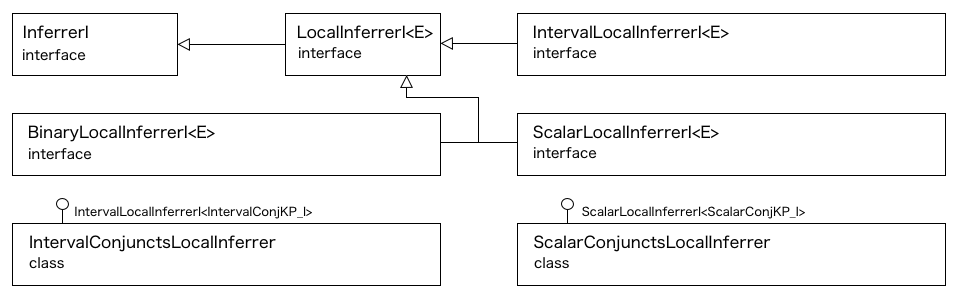
\includegraphics[width=\textwidth]{Inferrers}
\caption{Диаграмма структуры Inferer}
\label{Inf}
\end{center}
\end{figure}

В AlgBN Math Library для упрощения работы с АБС был внедрен парсер~\cite{nsmv_apr} пропозициональных формул. Если раньше приходилось строить характеристический вектор для поступающей формулы вручную, то на данном этапе в метод поступает формула в виде строки, а далее ее обрабатывает парсер, строя для нее характеристический вектор. Такая автоматизация позволяет избежать ошибок при построении характеристического вектора.

\subsubsection{Пример решения задачи априорного вывода для скалярных ФЗ}

Приведем пример вызова метода для осуществления априорного вывода в библиотеки для фрагмента знаний со скалярными оценками вероятности истинности и пропозициональной формулы $f_1 = x_0 \rightarrow x_1$:

\begin{lstlisting}[label=list1,caption={Пример решения задачи априорного вывода для скалярного ФЗ},escapeinside={(*}{*)}]
public void aprioriInferenceTest(){= 0.6;
ArrayAlphabet alphabet = new ArrayAlphabet(new string[] { "x0", "x1", "x2" });
double[] bound = { 1, 0.7, 0.5, 0.3 };
ScalarKnowledgePattern scKP = new ScalarKnowledgePattern(alphabet, Convert.ToInt64("11", 2), new double[][] { bound });
double result = scKP.aprioriInference("x0=>x1", 2);
}
\end{lstlisting}

Для рассматриваемой формулы парсер построит следующий характеристический вектор: $\chi_{f_1} = \left( \begin{array}{c}
1\\
1\\
0 \\
1
\end{array}  \right)$. Далее для него будет посчитан вектор ${\bf L}_{f_1} = \left( \begin{array}{c}
1\\
0\\
-1 \\
1
\end{array}  \right)$, который в последствии будет использован в уравнении априорного вывода. Результатом выполнения системы операторов будет вероятность формулы $p(f_1) = 0.6$.



Пример для фрагмента знаний со скалярными оценками вероятности истинности и пропозициональной формулы $f_2 = x_0 \vee x_1$:

\begin{lstlisting}[label=list1,caption={Пример решения задачи априорного вывода для скалярного ФЗ},escapeinside={(*}{*)}]
public void aprioriInferenceTest1()
{
double expectedResultLB = 0.9;
ArrayAlphabet alphabet = new ArrayAlphabet(new string[] { "x0", "x1", "x2" });
double[] bound = { 1, 0.8, 0.7, 0.6 };
ScalarKnowledgePattern scKP = new ScalarKnowledgePattern(alphabet, Convert.ToInt64("11", 2), new double[][] { bound });
double result = scKP.aprioriInference("x1|x0", 2)[0];    
Assert.AreEqual(expectedResultLB, result, 0.0001);

}
\end{lstlisting}

Для рассматриваемой формулы парсер построит следующий характеристический вектор: $\chi_{f_2} = \left( \begin{array}{c}
0\\
1\\
1 \\
1
\end{array}  \right)$. Далее для него будет посчитан вектор ${\bf L}_{f_2} = \left( \begin{array}{c}
0\\
1\\
1 \\
-1
\end{array}  \right)$, который в последствии будет использован в уравнении априорного вывода. Результатом выполнения системы операторов будет вероятность формулы $p(f_2) = 0.9$.


\subsubsection{Пример решения задачи априорного вывода для интервального ФЗ}
Пример для ФЗ с интервальными оценками вероятности истинности и пропозициональной формулы $f_3 = x_1 \leftrightarrow x_1$:

\begin{lstlisting}[label=list1,caption={Пример решения задачи априорного вывода для интервального ФЗ},escapeinside={(*}{*)}]
public void aprioriInferenceTest(){
double expectedResultLB = 0.46, expectedResultUB = 1;
ArrayAlphabet alphabet = new ArrayAlphabet(new string[] { "x0", "x1", "x2" });
double[] Lbound = { 1, 0.46, 0.29, 0.33 };
double[] Ubound = { 1, 0.7, 0.5, 0.9 };
IntervalKnowledgePattern intKP = new IntervalKnowledgePattern(alphabet, Convert.ToInt64("11", 2), new double[][] { Lbound, Ubound });
double[] result = intKP.aprioriInference("x0<=>x1", 2); 
}
\end{lstlisting}


Для рассматриваемой формулы парсер построит следующий характеристический вектор: $\chi_{f_3} = \left( \begin{array}{c}
1\\
0\\
0 \\
1
\end{array}  \right)$. Далее для него будет посчитан вектор ${\bf L}_{f_3} = \left( \begin{array}{c}
1\\
-1\\
-1 \\
2
\end{array}  \right)$, который в последствии будет использован в уравнении априорного вывода. В данном случае будет построена ЗЛП. Результатом выполнения системы операторов будет вероятность формулы $p(f_3) = [0.46, 1]$.




\subsection{Чувствительность}
%ПЕРЕХОД
Основным случаем анализа чувствительности локального апостериорного вывода в алгебраических байесовских сетях является анализ поведения оценки чувствительности $\epsilon$ первой задачи апостериорного вывода для фрагмента знаний~(ФЗ), построенного над идеалом конъюнктов, со скалярными оценками вероятности истинности и детерминированного свидетельства. Рассматривается допустимая вариация $\delta$ оценок фрагмента знаний в условиях фиксации исходного набора оценок ($\mathbf{P_{c}} = \mathbf{P_{c_0}}$).

Зададим ФЗ $(C, \mathbf{P_{c_0}})$ над алфавитом из двух атомов $A = \{ a_1, a_0 \}$. Следующий вектор состоит из скалярных оценок ФЗ:
\begin{equation*}
\Pc^{\circ} = \begin{pmatrix} 1 \\ p(x_1) \\ p(x_2) \\p(x_2x_1) \end{pmatrix} = \begin{pmatrix} 1 \\ 0.6 \\ 0.5 \\0.333 \end{pmatrix}. 
\end{equation*}

Для заданного ФЗ будем решать первую задачу апостериорного вывода со следующими детерминированными свидетельствами:
\begin{equation*}
\langle x_{1}\rangle;\langle ,x_{1}\rangle; \langle x_{2}\rangle;\langle x_{2}, x_{1} \rangle;  \langle x_{1}, x_{2} \rangle.
\end{equation*}

Перечисленные выше свидетельства соответствуют соответственно следующим пропозициональным формулам:
\begin{equation*}
x_{1}; \overline{x_{1}}; x_{2}; x_{2}\overline{x_{1}}; \overline{x_{2}}x_{1}.
\end{equation*}

Данным свидетельствам соответствуют следующие вектора-редистрибъютеры:
\begin{equation*}
\mathbf{r}^{\langle x_{1} \rangle} = \begin{pmatrix} 0 \\ 0 \\ 1 \\ 0 \end{pmatrix}; 
\mathbf{r}^{\langle x_{1} \rangle} = \begin{pmatrix} 1 \\ 0 \\ -1 \\ 0 \end{pmatrix};
\mathbf{r}^{\langle x_{2} \rangle} = \begin{pmatrix} 0 \\ 1 \\ 0 \\ 0 \end{pmatrix}; 
\end{equation*}
\begin{equation*}
\mathbf{r}^{\langle x_{2}, x_{1} \rangle} = \begin{pmatrix} 0 \\ 0 \\ 1 \\ -1 \end{pmatrix};
\mathbf{r}^{\langle x_{1}, x_{2} \rangle} = \begin{pmatrix} 0 \\ 1 \\ 0 \\ -1 \end{pmatrix}.
\end{equation*}
Для каждого свидетельства и и фиксированного $\delta$ (выбранной вариации вектора оценок вероятности истинности) вычислим оценку чувствительности $\epsilon$. Решим задачу линейного программирования~(ЗЛП) по поиску минимума и максимума следующего выражения:
\begin{equation*}
\p\evidence - \widehat{p}\evidence
\end{equation*}

\noindent при ограничениях:
\begin{equation}\label{eq:boundary1} \In \Pc\geq 0,\end{equation}
\begin{equation}\label{eq:boundary2} \Pc = \Pc^{\circ},    \end{equation}
\begin{equation}\label{eq:boundary3}\In \PcHat \geq 0,    \end{equation}
\begin{equation}\label{eq:boundary4} v(\Pc, \PcHat) \leq \delta,    \end{equation}
\begin{equation}\label{eq:boundary5}\p\evidence=(\redistributor,\Pc),     \end{equation}
\begin{equation}\label{eq:boundary6}\widehat{p}\evidence=(\redistributor,\PcHat),    \end{equation}
\begin{equation}\label{eq:boundary7} \PcHat[i] = 1.\end{equation}

В первом блоке~(\ref{eq:boundary1}) ограничений задаются условия на непротиворечивость оценок вероятности истинности элементов рассматриваемого вектора $\Pc$. 
С помощью второго блока~(\ref{eq:boundary2}) фиксируются скалярные оценки исходного вектора. 
В третьем блоке~(\ref{eq:boundary3}) задаются условия на непротиворечивость варьируемого вектора $\PcHat$. Четвертый~(\ref{eq:boundary4}) -- накладывает ограничения на вариативность. 
Следующие два ограничения~(\ref{eq:boundary5}, \ref{eq:boundary6}) задают то, каким образом решения первой задачи апостериорного вывода для фиксированного свидетельства и векторов $\Pc$ и $\PcHat$ выражаются через элементы этих векторов соответственно. Последнее условие~(\ref{eq:boundary7}) гарантирует нам выполнение необходимого условия того, что вероятность пустой конъюнкции в варьируемом векторе будет равна 1.

\begin{table}[htbp]
\caption{Оценки чувствительности для детерминированных свидетельств.} 
\begin{center}
\begin{tabular}{ |c|c|c|c|c|c|c|c|c| }
\hline
Свид-во &     $\delta= .01$ & $ .07$ & $ .15$ & $.27$ & $.43$ & $.58$ & $.7$ & $1$ \\ \hline
$\langle x_{2}, x_{1} \rangle$ & $.02$ & $.14$ & $.3$ & $.503$ & $.663$ & $.813$ & $.833$ & $.833$ \\
$\langle x_{2} \rangle$ & $.01$ & $.07$ & $.15$ & $.27$ & $.4$ & $.4$ & $.4$ & $.4$ \\
$\langle x_{1}, x_{2} \rangle$ & $.02$ & $.14$ & $.3$ & $.503$ & $.663$ & $.733$ & $.733$ & $.733$ \\
$\langle x_{1} \rangle$ & $.01$ & $.07$ & $.15$ & $.27$ & $.43$ & $.5$ & $.5$ & $.5$ \\
$\langle , x_{1} \rangle$ & $.01$ & $.07$ & $.15$ & $.27$ & $.43$ & $.5$ & $.5$ & $.5$ \\\hline
\end{tabular}
\end{center}
\label{tabular:sense}
\end{table}

В таблице \ref{tabular:sense} приведены оценки чувствительности для фиксированных дельт и набора рассматриваемых детерминированных свидетельств. На некоторых интервалах значений дельты прослеживается линейная зависимость дельты и получаемой оценки чувствительности. 

\begin{figure}[htbp]
\centerline{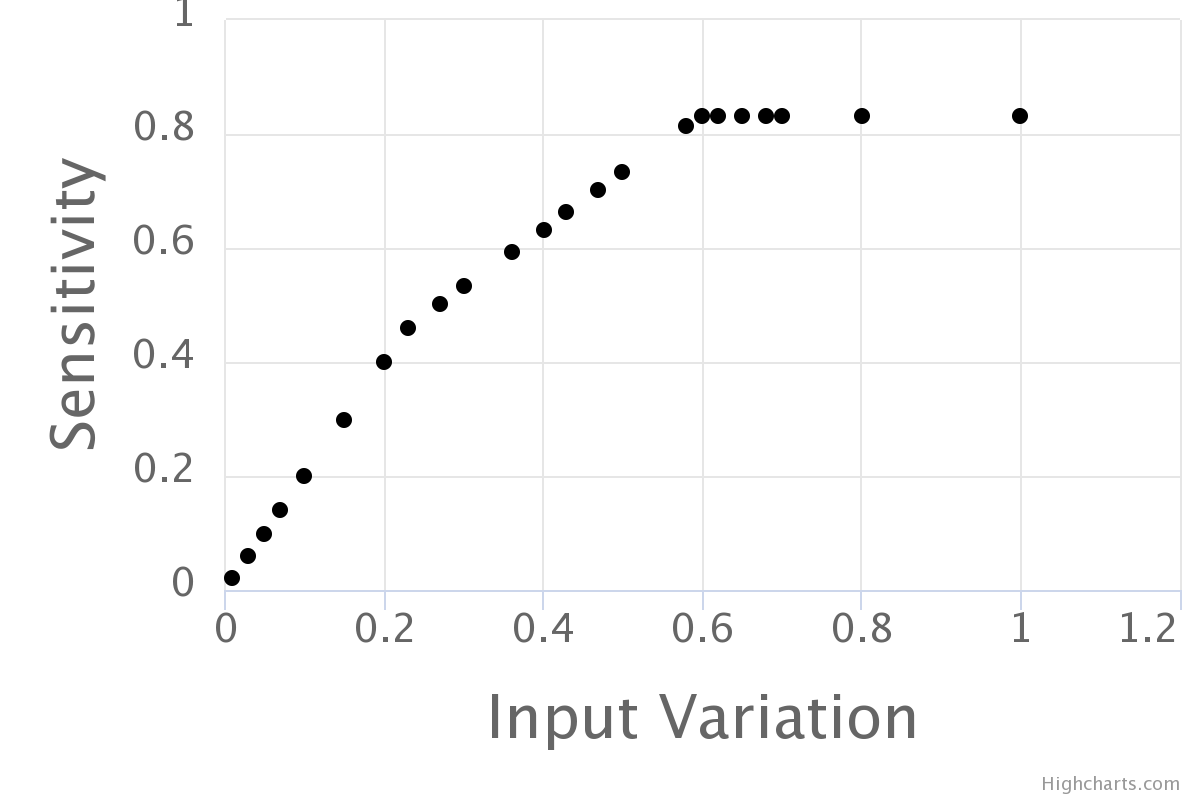
\includegraphics[width=0.8\textwidth]{chart_1.png}}
\caption{График оценок чувствительности для детерминированного свидетельства  $\langle x_{2}, x_{1} \rangle$}
\label{chart1}
\end{figure}

На рис.\ref{chart1} представлен график роста оценки чувствительности с ростом допустимой вариации исходного вектора в рамках рассматриваемой первой задачи апостериорного вывода для детерминированного свидетельства $\langle x_{2}, x_{1} \rangle$ и кванта $x_{2} \overline{x_{1}}$, в виде которого она может быть представлена.

\begin{figure}[htbp]
\centerline{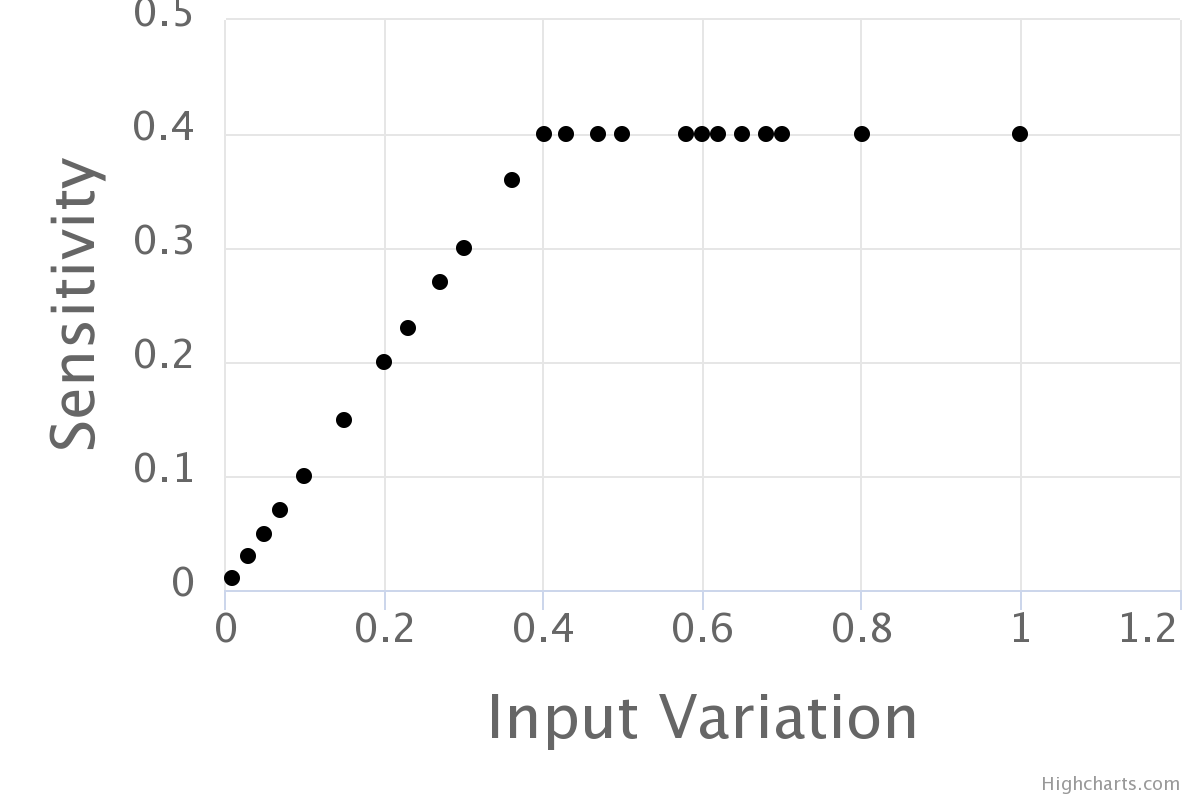
\includegraphics[width=0.8\textwidth]{chart_2.png}}
\caption{График оценок чувствительности для детерминированного свидетельства  $\langle x_{2} \rangle$}
\label{chart2}
\end{figure}

На рис.\ref{chart2} представлен график роста оценки чувствительности с ростом допустимой вариации исходного вектора в рамках рассматриваемой первой задачи апостериорного вывода для детерминированного свидетельства $\langle x_{2}\rangle$ и кванта $x_{2}$, в виде которого она может быть представлена.

\begin{figure}[htbp]
\centerline{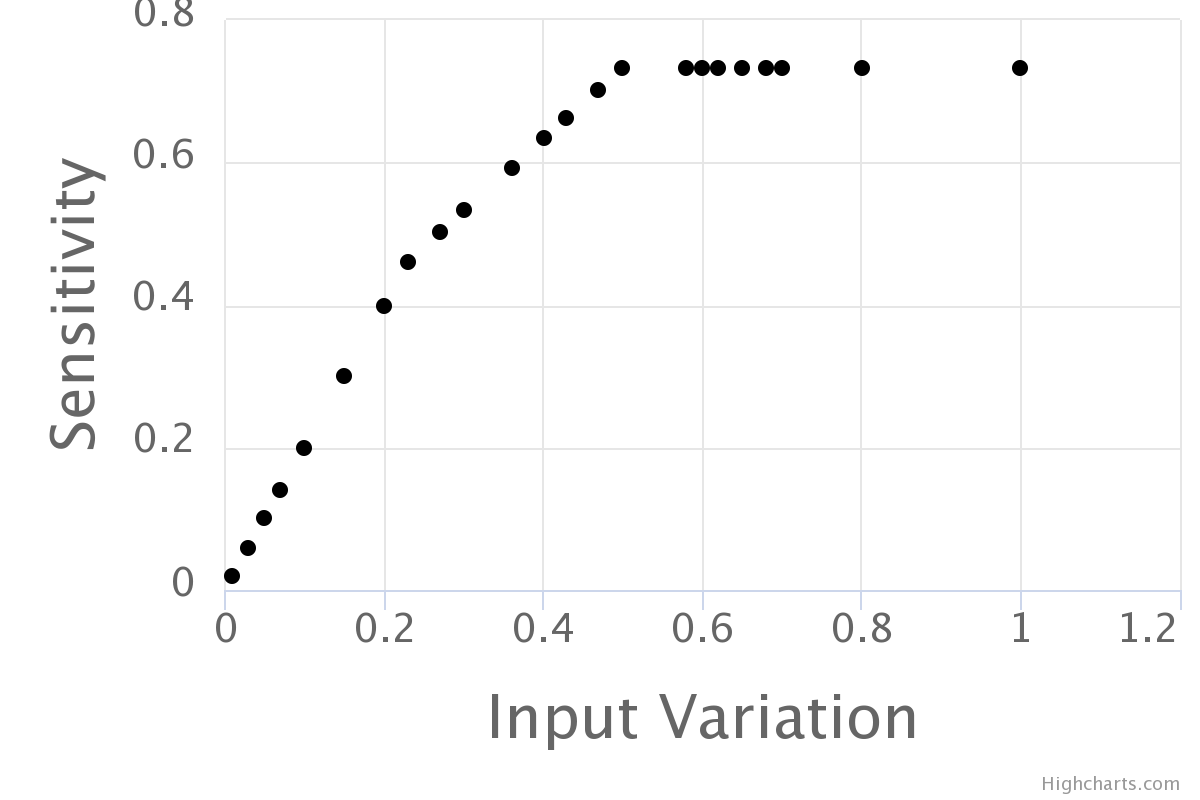
\includegraphics[width=0.8\textwidth]{chart_3.png}}
\caption{График оценок чувствительности для детерминированного свидетельства  $\langle x_{1}, x_{2} \rangle$}
\label{chart3}
\end{figure}

На рис.\ref{chart3} представлен график роста оценки чувствительности с ростом допустимой вариации исходного вектора в рамках рассматриваемой первой задачи апостериорного вывода для детерминированного свидетельства $\langle x_{1}, x_{2} \rangle$ и кванта $\overline{x_{2}} x_{1}$, в виде которого она может быть представлена.

\begin{figure}[htbp]
\centerline{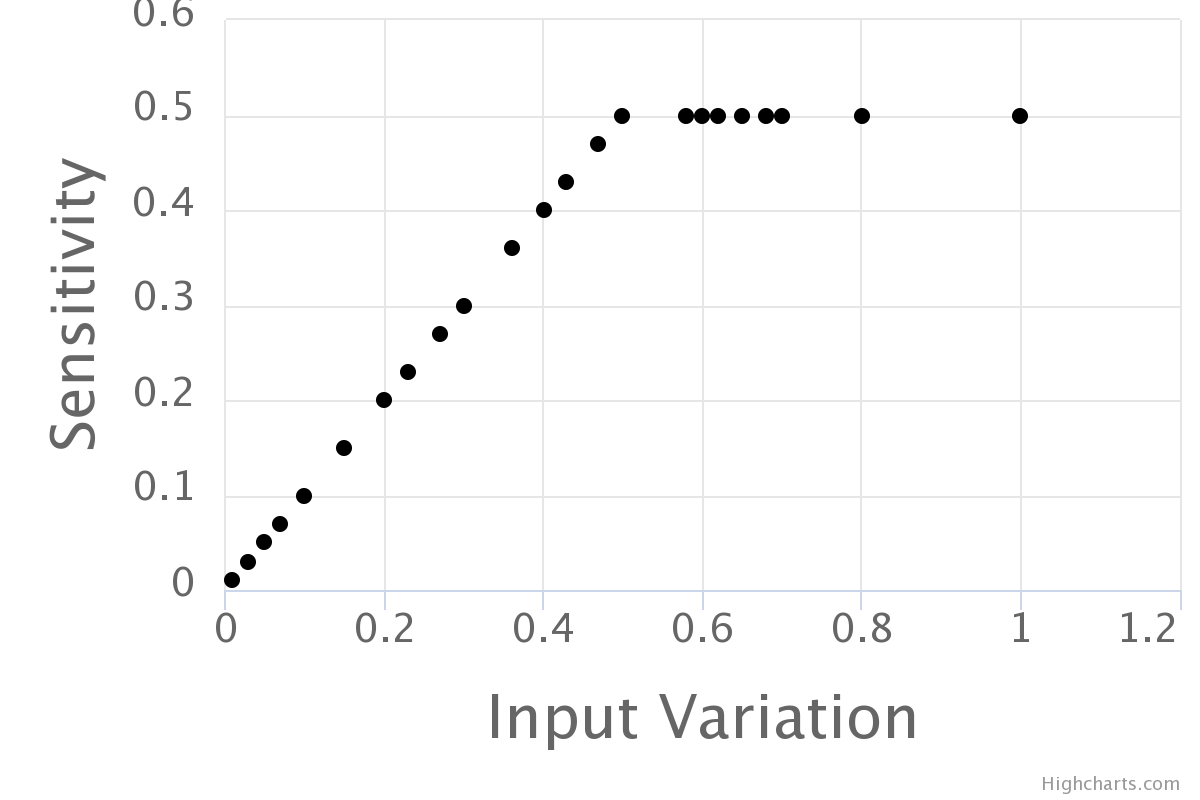
\includegraphics[width=0.8\textwidth]{chart_4.png}}
\caption{График оценок чувствительности для детерминированных свидетельств  $\langle  x_{1} \rangle$ и $\langle , x_{1} \rangle$}
\label{chart4}
\end{figure}

На рис.\ref{chart4} представлен график роста оценки чувствительности с ростом допустимой вариации исходного вектора в рамках рассматриваемой первой задачи апостериорного вывода для детерминированных свидетельств $\langle x_{1} \rangle$ и $\langle , x_{1} \rangle$, с квантами $x_{1}$ и $\overline{x_{1}}$ соответственно. Для обоих случаев график зависимости, как было показано экспериментально, совпал.

Как можно видеть из приведенных графиков, зависимость оценки чувствительности результата решения задачи первого вывода для представленных свидетельств выражается линейно на некоторых интервалах. Показано, что чувствительность возрастает при возрастании дельта, а потом стабилизируется.

    
\subsection{Выводы по главе}
 
    % Conclusion
    %%%%%%%%%%%%%%%%%%%%%%%%%%%%%%%%%%%%%%%
    \section*{Заключение}

   В ходе работы над магистерской диссертацией была достигнута основная цель -- проведен реинжениринг библиотеки для осуществления локального логико-вероятностного вывода над фрагментами знаний AlgBN Math Library. 
    
    Все задачи были выполнены, получены следующие результаты:
   \begin{enumerate}
                \item[1)] разработана система Unit-тестов для библиотеки AlgBN Math Library;
                \item[2)] спроектирована и реализована настройка в AlgBN Math Library для осуществления локального ЛВВ в применении в глобальных структурах;
                \item[3)] внедрен парсер в машину для априорного вывода в AlgBN Math Library;
                \item[4)] реализована система методов для проведения вычислительных экспериментов по вычислению оценки чувствительности первой задачи для детерминированного свидетельства и ФЗ со скалярными оценками в AlgBN Math Library.
   \end{enumerate}
    
    Результаты вошли в 15 публикаций:
    \begin{enumerate}
        \item	\textbf{Мальчевская~Е.А.} Архитектура библиотеки AlgBNModeller: представление альтернативных фрагментов знаний // Региональная информатика (РИ-2016). Юбилейная XV Санкт-Петербургская международная конференция «Региональная информатика (РИ-2016)». (Санкт-Петербург, 26-28 октября 2016 г.): Материалы конференции. СПб: СПОИСУ, 2016. С. 519;
		\item	Харитонов~Н.А., \textbf{Мальчевская~Е.А.}  Локальный априорный вывод в АБС: автоматизация анализа пропозициональной формулы// Региональная информатика (РИ-2016). Юбилейная XV Санкт-Петербургская международная конференция «Региональная информатика (РИ-2016)». (Санкт-Петербург, 26-28 октября 2016 г.): Материалы конференции. СПб: СПОИСУ, 2016. С. 522;
		\item	Золотин~А.А., \textbf{Мальчевская~Е.А.}, Бирилло~А.И., Тулупьев~А.Л. Управление согласованностью оценок вероятностей в локальном апостериорном выводе в алгебраических байесовских сетях // 9-я Российская мультиконференция по проблемам управления, материалы 9-й конференции "Информационные технологии в управлении" (ИТУ-2016) - СПб: АО "Концерн "ЦНИИ "Электроприбор", 2016, С. 52-61;
        \item Золотин А.A., Левенец Д.Г., \textbf{Мальчевская Е.А.}, Зотов М.А., Бирилло А.И., Березин А.И., Иванова А.В., Тулупьев А.Л. Алгоритмы обработки и визуализации алгебраических байесовских сетей // Образовательные технологии и общество. 2017. Т.20. №1. С.446-457;
        \item	\textbf{Мальчевская Е.А.} Имплементация уравнений локального логико- вероятностного вывода в комплексе программ AlgBN Math Library //  Нечеткие системы, мягкие вычисления и интеллектуальные технология (НСМВИТ-2017) труды VII всероссийской научной-практической конференции. 2017. С. 125-134;
        \item	\textbf{Мальчевская Е.А.}, Бирилло А.И., Харитонов Н.А., Золотин А.А. Развитие матрично-векторного подхода в алгоритмах локального априорного вывода в алгебраических байесовских сетях // Нечеткие системы, мягкие вычисления и интеллектуальные технология (НСМВИТ-2017) труды VII всероссийской научной-практической конференции. 2017. С. 92-100; 
        \item	\textbf{Мальчевская Е.А.} Алгоритмизация локального апостериорного логико-вероятностного вывода в алгебраических байесовских сетях // Интеллектуальные системы и технологии: современное состояние и перспективы Сборник научных трудов IV Международной летней школы-семинара по искусственному интеллекту для студентов, аспирантов, молодых ученых и специалистов. 2017. С. 120-127;
        \item	Zolotin, A. A., \textbf{Malchevskaya, E. A.}, Tulupyev, A. L., Sirotkin, A. V. (2017, September). An Approach to Sensitivity Analysis of Inference Equations in Algebraic Bayesian Networks. In International Conference on Intelligent Information Technologies for Industry (pp. 34-42). Springer, Cham;
        \item	\textbf{Мальчевская Е.А.}, Золотин А.А., Тулупьев А.Л. Уравнения апостериорного вывода в фрагментах знаний над идеалом дизъюнктов // Всероссийская научная конференция по проблемам информатики (СПИСОК-2017). (Санкт-Петербург, 25-27 апреля 2017 г.). Санкт-Петербург: СПбГУ, 2017. C. 395-403.
        \item	\textbf{Мальчевская Е.А.} Анализ чувствительности локального логико-вероятностного вывода в математической библиотеке AlgBN Math Library. // Информационная безопасность регионов России (ИБРР-2017). X Санкт-Петербургская межрегиональная конференция. (Санкт-Петербург, 1–3 ноября 2017 г.): Материалы конференции. СПб: СПОИСУ, 2017. С. 423–424;
        \item \textbf{Мальчевская Е.А.}, Золотин А.А., Тулупьев А.Л. Алгоритмы апостериорного вывода в алгебраических байесовских сетях: рафинирование матрично-векторного представления // Нечеткие системы и мягкие вычисления. Промышленные применения. Fuzzy Technologies in the Industry (FTI-2017): Первая Всероссийская научно-практическая конференция (Россия, г. Ульяновск, 14-15 ноября, 2017 г.): сборник научных трудов. – Ульяновск : УлГТУ, 2017. 376-388 с;
        \item	\textbf{Malchevskaya E.}, Kharitonov N., Zolotin A., Birillo A. Algebraic Bayesian Networks: Probabilistic-Logic Inference Algorithms and Storage Structures // Proceedings of the Finnish-Russian University Cooperation in Telecommunications(FRUCT’20) Conference, 2017. P 628-633;
        \item	Тулупьев А.Л., Тулупьева Т.В., Суворова А.В., Абрамов М.В., Золотин А.А., Зотов М.А., Азаров А.А.,\textbf{ Мальчевская Е.А.}, Левенец Д.Г., Торопова А.В., Харитонов Н.А., Бирилло А.И., Сольницев Р.И., Микони С.В., Орлов С.П., Толстов А.В. Мягкие вычисления и измерения. Модели и методы: монография. Том III / под ред. д.т.н., проф. С.В. Прокопчиной. – М.: ИД "НАУЧНАЯ БИБЛИОТЕКА", 2017. – 300 с;
        \item	жНСМВ!
        \item	ТвГТУ
        \end{enumerate}
    
  Результаты были представлены на восьми конференциях: 
  \begin{enumerate}
                \item  РИ’2016: Юбилейная XV Санкт-Петербургская международная конференция «Региональная информатика 2016». Темы докладов: «Архитектура библиотеки AlgBNModeller: представление альтернативных фрагментов знаний» и «Локальный априорный вывод в алгебраических байесовских сетях: автоматизация анализа пропозициональной формулы». Санкт-Петербург, 26-28 октября 2016 г.;
                \item	IITI-2017: 2nd International Scientific Conference “Intelligent infor\-ma\-tion technologies for industry” (IITI’17). Варна, Болгария, 14–16 сентября 2017;
                \item	Всероссийская научная конференция по проблемам информатики СПИСОК–2017. Санкт-Петербург, 25–27 апреля 2017;
                \item	FTI’2017: Первая всероссийская научно-практическая конференция «Нечеткие системы и мягкие вычисления. Промышленные применения» (Fuzzy Technologies in the Industry – FTI-2017). Ульяновск, 14–15 ноября 2017;
                \item	НСМВИТ’2017: VII-я Всероссийская научно-практическая конференция «Нечеткие системы, мягкие вычисления и интеллектуальные технологии» (НСМВИТ-2017). Санкт-Петербург, 3–7 июля 2017;
                \item	ISyT’2017: IV-я Международная летняя школа-семинар по искусственному интеллекту для студентов, аспирантов, молодых ученых и специалистов «Интеллектуальные системы и технологии: современное состояние и перспективы–2017» (ISyT–2017). Санкт-Петербург, 30 июня – 3 июля 2017;
                \item	ИБРР’2017: X Санкт-Петербургская межрегиональная конференция «Информационная безопасность регионов России (ИБРР-2017)». Санкт-Петербург, 1–3 ноября 2017;
                \item   FRUCT’2017: 20th Finnish-Russian University Cooperation in Te\-le\-commu\-ni\-ca\-tions (FRUCT) Conference. Санкт-Петербург, 5-7 апреля 2017;
   \end{enumerate}
    
   Была подана заявка на регистрацию программы для ЭВМ: Мальчевская~Е.А., Тулупьев~А.Л. Algebraic Bayesian Network Local Reconciler, Version 01 for CSharp (AlgBN L Reconciler cs.v.01).

	Работа выполнялась под руководством А.Л.~Тулупьева, на базе лаборатории теоретических и междисциплинарных проблем информатики СПИИРАН в рамках проекта по государственному заданию № 0073-2014-0002; кроме того, разработки были частично поддержаны грантами РФФИ 15-01-09001-a~--- <<Комбинированный логико-ве\-роят\-ност\-ный графический подход к представлению и обработке систем знаний с неопределенностью: алгебраические байесовские сети и родственные модели>>, 18-01-00626~--- <<Методы представления, синтеза оценок истинности и машинного обучения в алгебраических байесовских сетях и родственных моделях знаний с неопределенностью: логико-вероятностный подход и системы графов>>.
    
   % Полученные результаты позволяют в будущем развить функциональность данной библиотеки, реализовывать глобальный логико-ве\-ро\-ятност\-ный вывод, а также интегрироваться с другими подпроектами, которые связаны со структурной компонентой библиотеки.  
   
\setmonofont[Mapping=tex-text]{CMU Typewriter Text}
\bibliographystyle{ugost2008ls}   
% Bibliography (CHANGE)
    %%%%%%%%%%%%%%%%%%%%%%%%%%%%%%%%%%%%%%%
  %  \input{biblio}
%\bibliography{diploma.bib}
\end{document}
